\chapter{Podatki in metode}
\section{Razvojno okolje MATLAB}
Ves razvoj je potekal v programskem okolju MATLAB. Ta poleg samega programskega jezika vsebuje velik nabor že implementiranh funkcij, napredne aplikacije za strojno učenje in knjižnice ki omogočajo povezave z laboratorijskimi napravami. V njem sta ustvarjeni funkciji za računanje matrik Grangerjevega indeksa vzročnosti
in matrik Kompleksnega Pearsonov korelacijskega koeficienta, prav tako so v njem ustvarjene nevronske mreže in uporabljeno je za ostala razvrščanja in funkcijo za zajemanje podatkov iz naprave Cognionics Quick-20 ter funkcijo ki v realnem času razpoznava gibanje. \cite{MATLAB}
\begin{figure}[h!]
    \begin{center}
    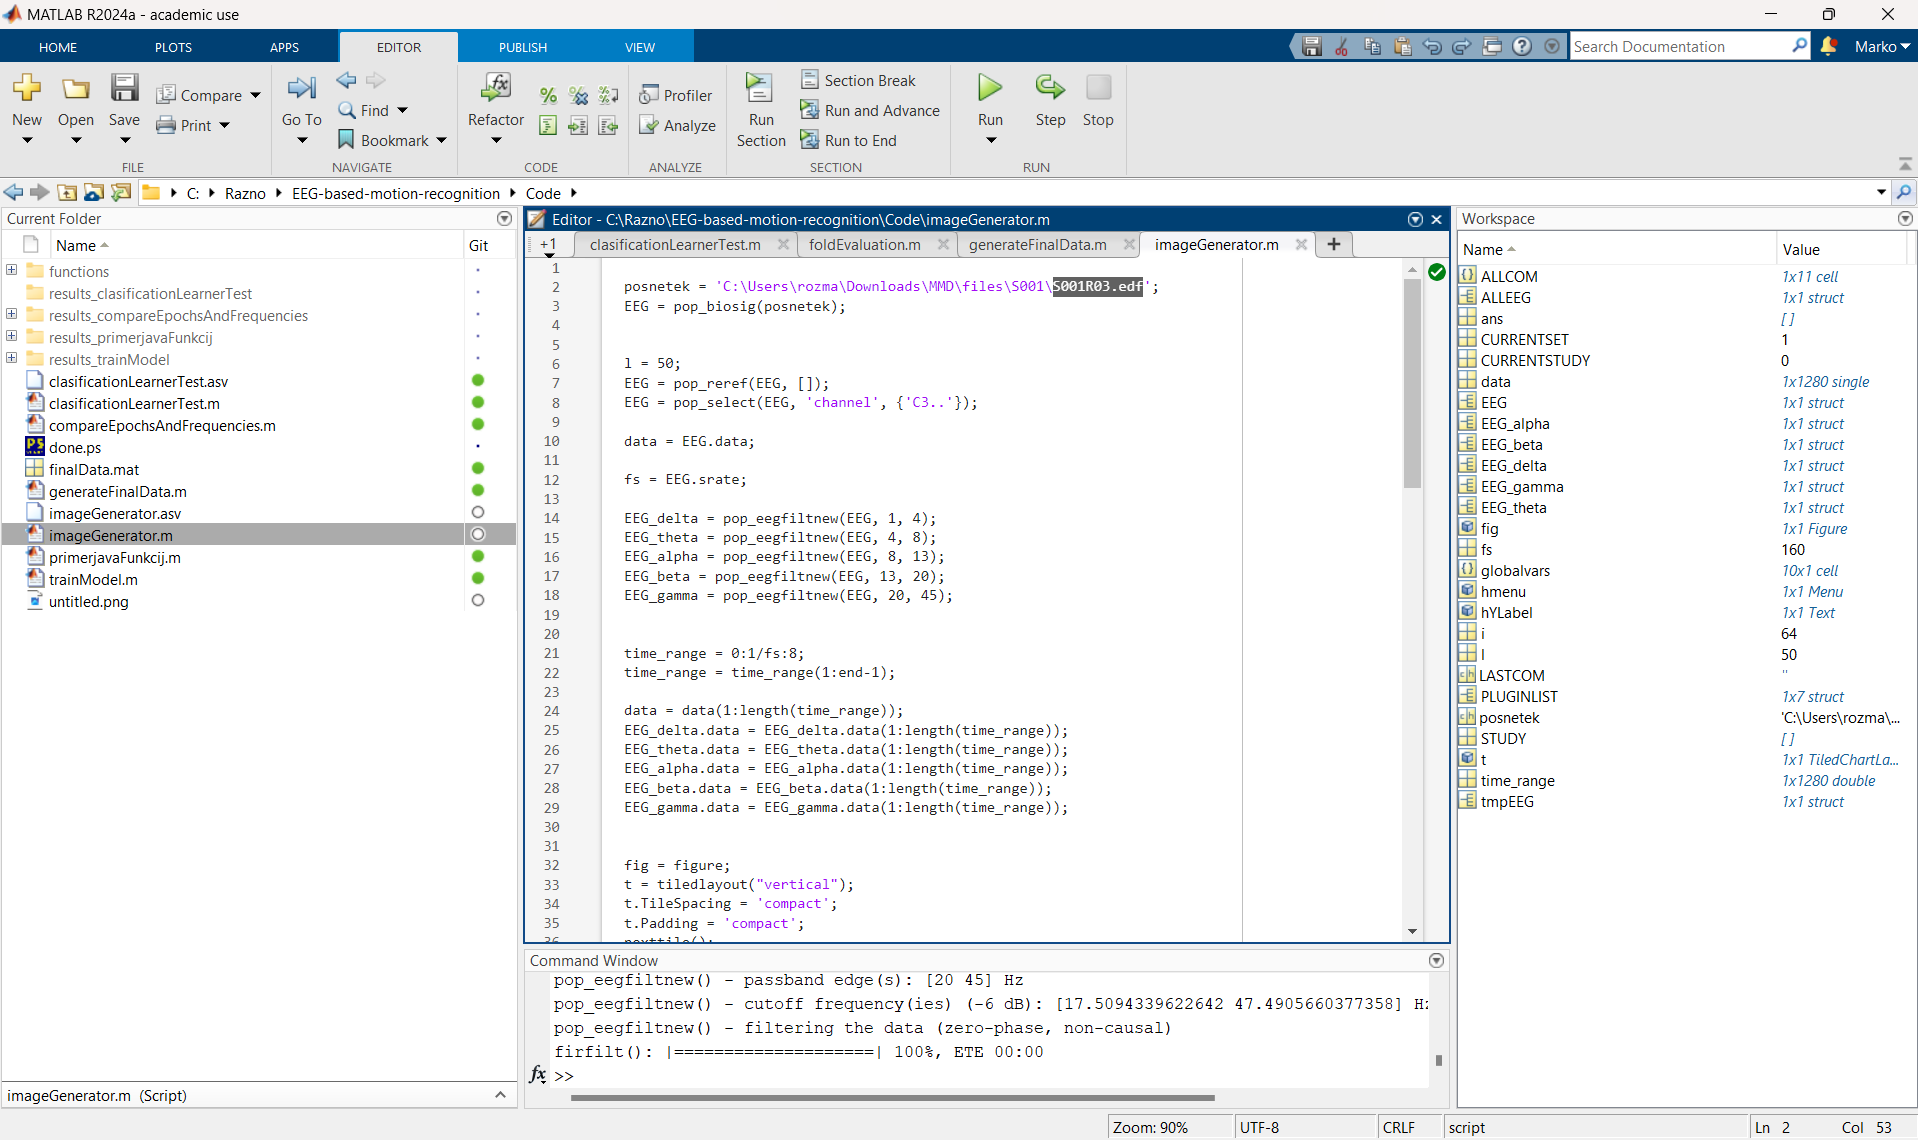
\includegraphics[width=1\linewidth]{slike/Matlab.png}
    \end{center}
    \caption{Programsko okolje MATLAB. Od leve proti desni: podokno z datotekami, podokno s kodo, podokno s spremenljivkami. Zgoraj zavihki za orodjarno, aplikacije in prikaz podatkov.}
    \end{figure}
    
\subsection{EEGLAB}
EEGLAB je interaktivna matlab orodjarna, za procesiranje in obdelavo elektrofizioloških podatkov. Omogoča rereferenciranje EEG signalov, izbiro določenih elektrod, deljenje podatkov na epohe glede na dogodke in filtriranje frekvenc. Omogoča interakcijo preko uporabniškega vmesnika. Vse akcije v vmesniku se prevedejo v ukaze. Grafični vmesnik je uporaben za enostavne analize. Za avtomatizacijo pa njegove funkcije uporabimo v svoji kodi z ustreznimi ukazi. Pri izdelavi naloge smo največ uporabljali funkcije branja .edf datotek, filtriranja frekvenc signalov in deljenja posnetkov na manjše dele.\cite{EEGLAB}
\begin{figure}[h!]
    \begin{center}
    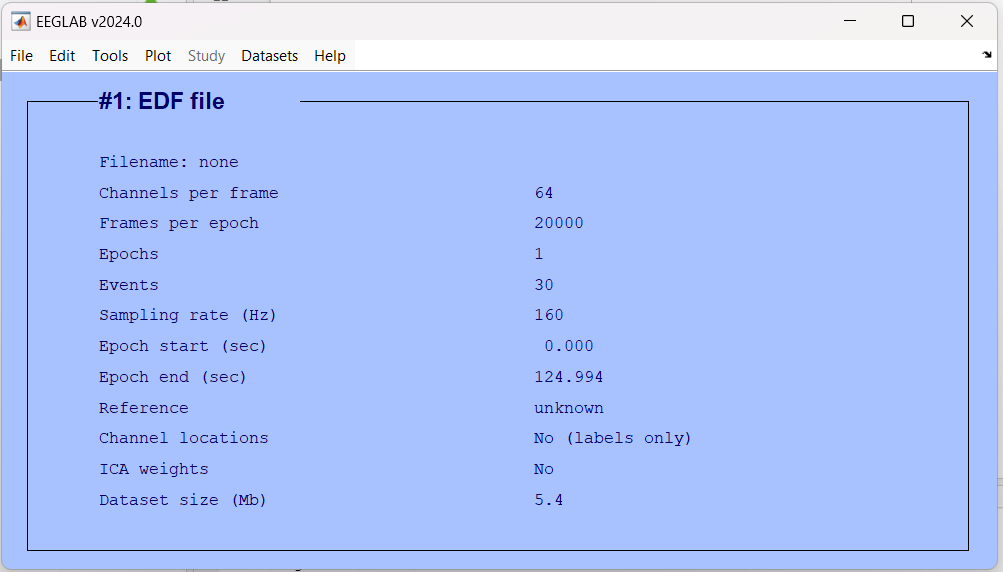
\includegraphics[width=1\linewidth]{slike/EEGLAB.png}
    \end{center}
    \caption{Orodjarna eeglab. Zgoraj zavihki za delo z datotekami, urejanje, orodja, prikaz podatkov, delo z zbirkami podatkov in pomoč. Naložen podatkovni niz dolžine 124 sekund z 30 dogodki.}
    \end{figure}

\subsection{Lab streaming layer}
Lab streaming layer je odprtokodna vmesna programska oprema ki omogoča pošiljanje, prejemanje, sinhronizacijo in snemanje tokov podatkov znotraj lokalnega omrežja. Med drugim je na voljo v obliki MATLAB knjižnice, ki omogoča preprosto integracijo EEG naprav s programsko opremo MATLAB. Knjižnico je potrebno prenesti in nato zgraditi na svojem računalniku.  \cite{Lslwebsite}

\subsection{Classification learner}
Classification learner je aplikacija v okolju MATLAB za enostavno razvrščanje podatkov. Podpira različne metode razvrščanja, prečno preverjanje in uporabo različnih podatkov za gradnjo in testiranje modela. Aplikacija podpira razvrščanje podatkov iz dvo dimenzionalnih matrik kjer vrstice ali stolpci predstavljajo spremenljivke. Oznake podatkov lahko podamo kot določeno vrstico ali stolpec matrike ali v ločeni spremenljivki. Zaradi omejitev aplikacije smo pred razvrščanjem matrike povezljivosti pretvorili v vektorje in te združili v matriko podatkov. Z aplikacijo smo lahko hitro ocenili uspešnost računanja matrik povezljivosti in primerjali delovanje različnih razvrščanj v primerjavi z našo nevronsko mrežo.
\begin{figure}[h!]
    \begin{center}
    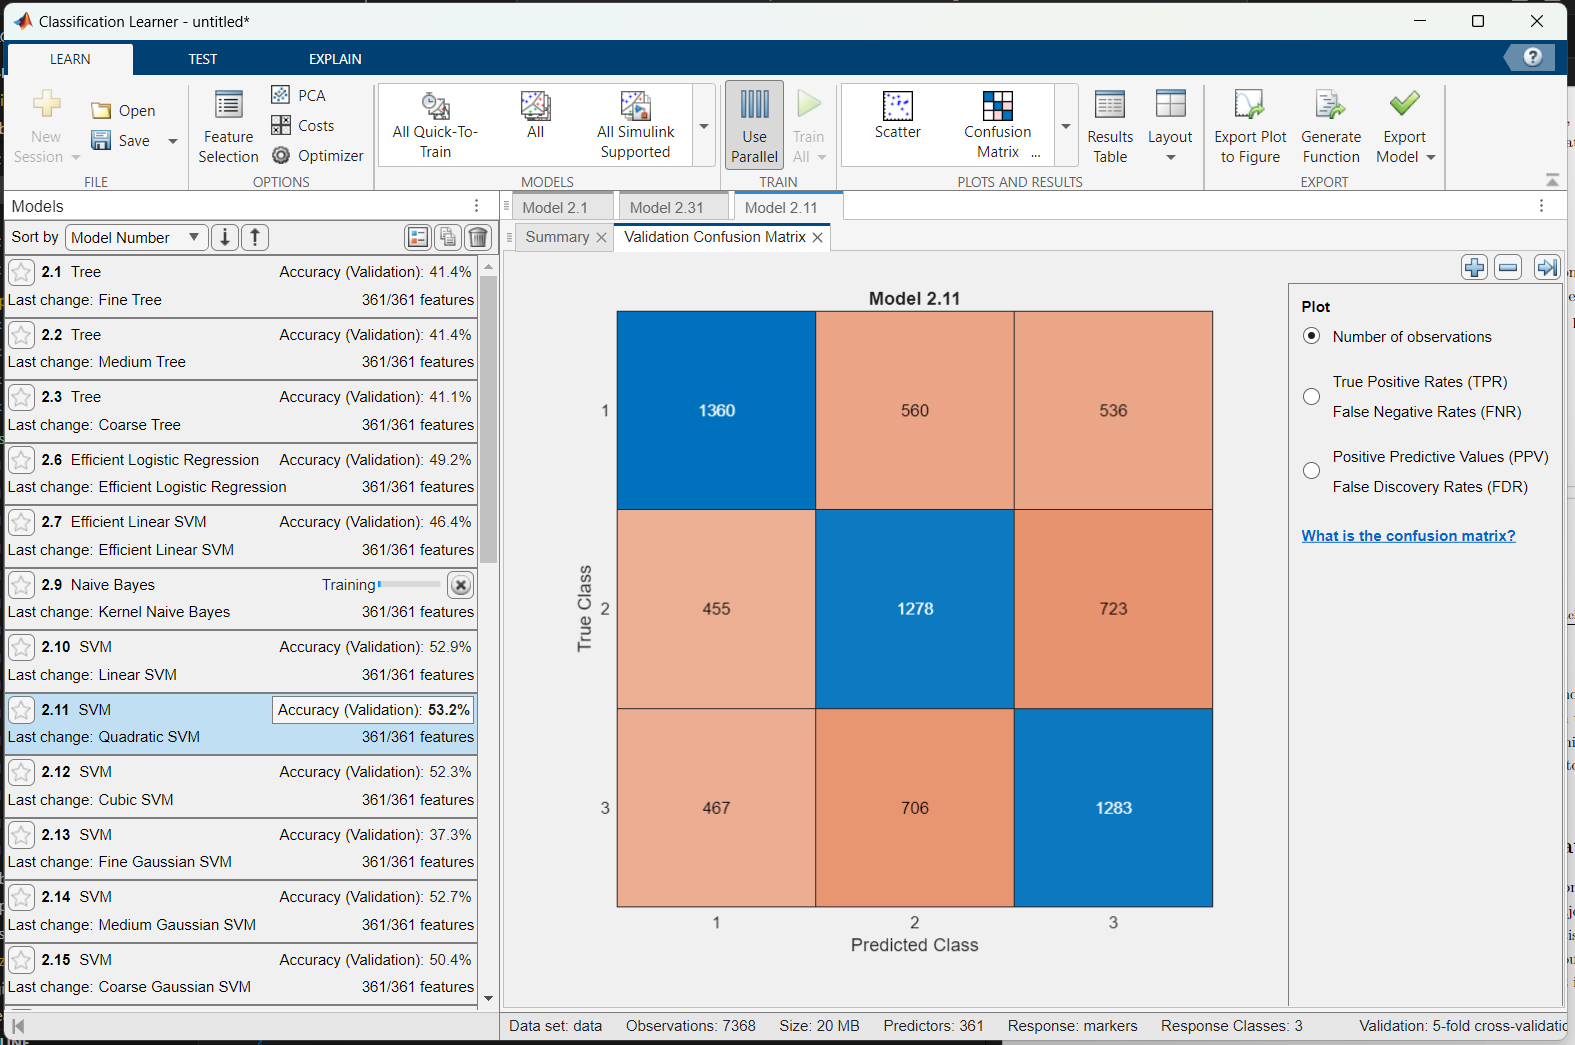
\includegraphics[width=1\linewidth]{slike/ClasificationLearner.png}
    \end{center}
    \caption{Aplikacija classification learner. Na levi strani podokno z različnimi metodami razvrščanja, na sredini prikaz podrobnosti izbrane metode. Zgoraj zavihki za učenje, testiranje in razlago. }
    \end{figure}

\section{Podatkovna zbirka\\ EEG Motor Movement/Imagery Dataset}
EEG Motor Movement/Imagery Dataset(MMID) je prosto dostopna zbirka več kot 1500 eno in dve minutnih posnetkov 109 prostovoljcev. Zbirka za vsakega prostovoljca vsebuje dva izhodiščna posnetka in po tri posnetke opravljanja štirih različnih nalog: stiskanje in sproščanje leve ali desne pesti(naloga 1), namišljeno stiskanje in sproščanje leve ali desne pesti(naloga 2), stiskanje in sproščanje obeh pesti ali obeh stopal(naloga 3), namišljeno stiskanje in sproščanje obeh pesti ali obeh stopal(naloga 4). Za nas relevantni so posnetki serij 3, 7 in 11 v katerih prostovoljci opravljajo prvo nalogo. Posnetki so shranjeni v formatu EDF+ ki vsebuje posnetke EEG in oznake dogodkov. Snemanje je bilo opravljeno z sistemom BCI2000 z 64 elektrodami postavljenimi po mednarodnem sistemu 10-10(slika \ref{slika:mednarodni_sistem_10}) brez elektrod Nz, F9, F10, FT9, FT10, A1, A2, TP9, TP10, P9, in P10.\cite{schalkBCI2000GeneralpurposeBraincomputer2004,schalkEEGMotorMovement2009}

\begin{table}[h]
\centering
\begin{tabular}{|c|c|l|}

\hline
Številka serije & Naloga &Opis naloge \\
\hline
1 & izhodišče & odprte oči  \\
\hline
2 & izhodišče & zaprte oči  \\
\hline
3 & naloga 1 & stiskanje in sproščanje leve ali desne pesti \\
\hline
4 & naloga 2 &namišljeno stiskanje in sproščanje leve ali desne pesti  \\
\hline
5 & naloga 3 &stiskanje in sproščanje obeh pesti ali obeh stopal \\
\hline
6 & naloga 4 &namišljeno stiskanje in sproščanje obeh pesti ali obeh stopal  \\
\hline
7 & naloga 1 &stiskanje in sproščanje leve ali desne pesti \\
\hline
8 & naloga 2 &namišljeno stiskanje in sproščanje leve ali desne pesti  \\
\hline
9 & naloga 3 &stiskanje in sproščanje obeh pesti ali obeh stopal \\
\hline
10 & naloga 4 &namišljeno stiskanje in sproščanje obeh pesti ali obeh stopal  \\
\hline
11 & naloga 1 &stiskanje in sproščanje leve ali desne pesti \\
\hline
12 &naloga 2 &namišljeno stiskanje in sproščanje leve ali desne pesti  \\
\hline
13 & naloga 3 &stiskanje in sproščanje obeh pesti ali obeh stopal \\
\hline
14 & naloga 4 &namišljeno stiskanje in sproščanje obeh pesti ali obeh stopal  \\

\hline
\end{tabular}
\caption{Naloge in opisi nalog, ki jih prostovoljci opravljajo v posnetkih zbirke podatkov MMID.}
\end{table}


\section{Metode povezljivosti}
Metode povezljivosti se uporabljajo za analizo delovanja možganov, saj nam v nasprotju z direktnim razvrščanjem EEG signalov omogočajo identifikacijo specifičnih vzorcev. S tem pridobimo globlji vpogled v delovanje možganov.

\subsection{Grangerjev indeks vzročnosti}
Grangerjev indeks vzročnosti je statistična metoda za preverjanje, ali ena časovna vrsta nosi informacije o drugi. Metoda je bila razvita v šestdesetih letih devetnajstega stoletja za uporabo ekonomiji.\cite{cohenAnalyzingNeuralTime2014}

Za dve časovni vrsti $X_1$ in $X_2$ ter $p$ kot število prejšnjih vrednosti, ki jih upoštevamo pri računanju, lahko izračunamo $E_1$ in $E_1$ ki so napake pri predvidevanju naslednje vrednosti v vrsti $X_1$. V kolikor je varianca vrednosti $E_2$ manjša kot varianca vrednosti $E_1$ lahko predvidevamo, da časovna vrsta $X_2$ nosi informacije o časovni vrsti $X_1$. $A_1$, $A_2$ in $A_3$ so koeficienti avto-regresivnega modela. \cite{sethGrangerCausality2007}
\begin{align*}
X_1(t) &= \sum_{j=1}^{p} A_{1,j} X_1(t-j) + E_1(t)\\
X_1(t) &= \sum_{j=1}^{p} A_{2,j} X_1(t-j) + \sum_{j=1}^{p} A_{3,j} X_2(t-j) + E_2(t)
\end{align*}


\subsection{Kompleksni Pearsonov korelacijski koeficient}
Pearsonov korelacijski koeficient je najpogosteje uporabljen linearni korelacijski koeficient. Zanj smo se odločili saj v članku  \citetitle{sverkoComplexPearsonCorrelation2022}
avtorji pokažejo da vsebuje informacije Phase Locking Value(PLV) in Weighted Phase Lag Index(wPLI) ki sta dve najbolj pogosto uporabljeni metodi povezljivosti. V praksi nam pove, v kakšni meri sta fazi dveh signalov linearno povezani.\cite{sverkoComplexPearsonCorrelation2022} 

Ker želimo opazovati faze EEG signala, ga potrebujemo pretvoriti v analitični signal ki vsebuje informacijo o fazi. Zaradi sledeče transformacijo, ki je definirana samo na ozkih frekvenčnih pasovih potrebujemo signale EEG predhodno filtrirati. Analitični signal $X_a$ kjer $HT(X(t))$ označuje Hilbertovo transformacijo signala $X$.\cite{sverkoComplexPearsonCorrelation2022} 
\begin{align*}
    X_a(t) = X(t) + i \cdot HT(X(t))
\end{align*}

Za računanje Kompleksnega Pearsonovega korelacijskega koeficienta v našem primer lahko uporabimo naslednjo enačbo kjer sta $X_1$ in $X_2$ analitična signal dolžine $N$. $\overline{X_2(n)}$ pa konjugirana vrednost $X_2(n)$\cite{sverkoComplexPearsonCorrelation2022} 
\begin{align*}
r(X_1, X_2) &= \frac{\sum\limits_{n=1}^{N}(X_1(n) \cdot \overline{X_2(n)})}{\sqrt{\sum\limits_{n=1}^{N} |X_1(n)|^2} \cdot \sqrt{\sum\limits_{n=1}^{N} |X_2(n)|^2}}
\end{align*}

\section{Razvrščanje}
Želeli smo preizkusiti kako uspešno bi razvrščanje delovala na podatkih zbirke in kako uspešno bi delovala na naših podatkih, zato smo razvrščanje izvajali dvakrat. Enkrat na podatkih zbirke in enkrat na naših podatkih. Ker nevronska mreža za učenje potrebuje več podatkov kot jih lahko zagotovimo iz naših posnetkov smo jo za namene razvrščanja naših posnetkov naučili na podatkih MMID in nato dodatno naučili na naših podatkih. 

\subsection{Razvrščanje v okolju Classification learner}
Na matrikah povezljivosti pridobljenih iz podatkov zbirke in naših posnetkov smo izvedli več različnih vrst razvrščanja in sicer: odločitvena drevesa, metodo k najbližjih sosedov (k-NN), logistično regresijo, podporne vektorske stroje (SVM), ansabelske metode in nevronske mreže.


\subsection{Razvrščanje z lastno nevronsko mrežo}
Nevronska mreža je sestavljena iz vhodne plasti za slike dimenzij 19x19x1, polno povezane plasti s 100 nevroni, Leaky ReLU(usmerjena linearna enota) plasti, dropout(izpust) plasti z 50\% verjetnostjo izpustitve nevronov, polno povezane plasti z 10 nevroni, GELU plasti, dropout(izpust) plasti z 50\% verjetnostjo izpustitve nevronov, polno povezane plasti s tremi nevroni in softmax plasti. Mreža je realizirana z pomočjo MATLAB orodjarne Deep Learning Toolbox. Lastna implementacija nevronske mreže nam omogoča enostavnejšo interpretacijo podatkov in nudi možnost podrobnejše nadaljnje analize.
\begin{figure}[h!]
\begin{center}
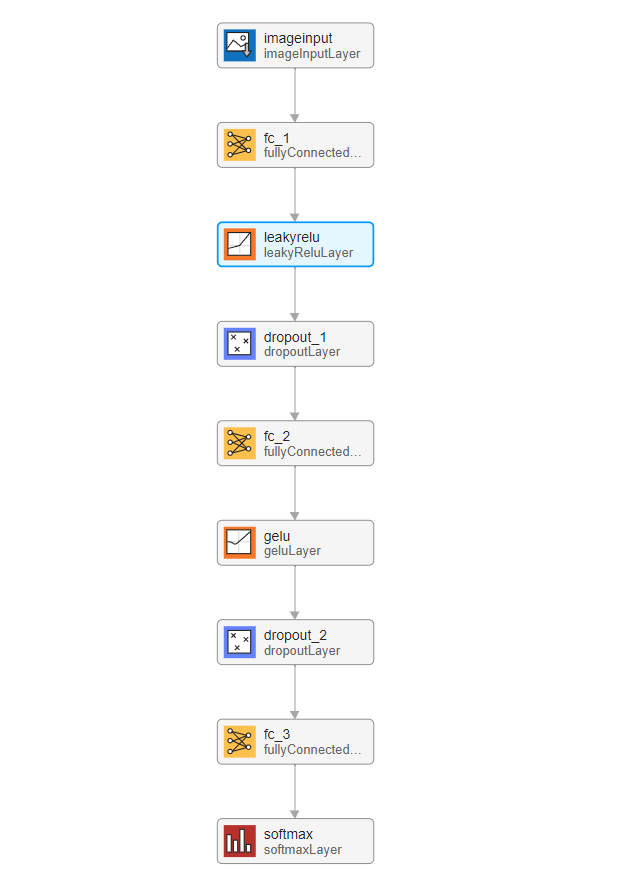
\includegraphics[width=0.8\linewidth]{slike/Neural network.png}
\end{center}
\caption{Arhitektura nevronske mreže v MATLAB aplikaciji Deep Network Designer. Od zgoraj navzdol: plast za slike, polno povezana, Leaky ReLU(usmerjena linearna enota), dropout(izpust), polno povezana, GELU, dropout(izpust), polno povezana in Softmax.}
\end{figure}






